%\VignetteIndexEntry{Example evaluation of FOCUS dataset Z}
%\VignetteEngine{knitr::knitr}
\documentclass[12pt,a4paper]{article}\usepackage[]{graphicx}\usepackage[]{color}
%% maxwidth is the original width if it is less than linewidth
%% otherwise use linewidth (to make sure the graphics do not exceed the margin)
\makeatletter
\def\maxwidth{ %
  \ifdim\Gin@nat@width>\linewidth
    \linewidth
  \else
    \Gin@nat@width
  \fi
}
\makeatother

\definecolor{fgcolor}{rgb}{0.345, 0.345, 0.345}
\newcommand{\hlnum}[1]{\textcolor[rgb]{0.686,0.059,0.569}{#1}}%
\newcommand{\hlstr}[1]{\textcolor[rgb]{0.192,0.494,0.8}{#1}}%
\newcommand{\hlcom}[1]{\textcolor[rgb]{0.678,0.584,0.686}{\textit{#1}}}%
\newcommand{\hlopt}[1]{\textcolor[rgb]{0,0,0}{#1}}%
\newcommand{\hlstd}[1]{\textcolor[rgb]{0.345,0.345,0.345}{#1}}%
\newcommand{\hlkwa}[1]{\textcolor[rgb]{0.161,0.373,0.58}{\textbf{#1}}}%
\newcommand{\hlkwb}[1]{\textcolor[rgb]{0.69,0.353,0.396}{#1}}%
\newcommand{\hlkwc}[1]{\textcolor[rgb]{0.333,0.667,0.333}{#1}}%
\newcommand{\hlkwd}[1]{\textcolor[rgb]{0.737,0.353,0.396}{\textbf{#1}}}%
\let\hlipl\hlkwb

\usepackage{framed}
\makeatletter
\newenvironment{kframe}{%
 \def\at@end@of@kframe{}%
 \ifinner\ifhmode%
  \def\at@end@of@kframe{\end{minipage}}%
  \begin{minipage}{\columnwidth}%
 \fi\fi%
 \def\FrameCommand##1{\hskip\@totalleftmargin \hskip-\fboxsep
 \colorbox{shadecolor}{##1}\hskip-\fboxsep
     % There is no \\@totalrightmargin, so:
     \hskip-\linewidth \hskip-\@totalleftmargin \hskip\columnwidth}%
 \MakeFramed {\advance\hsize-\width
   \@totalleftmargin\z@ \linewidth\hsize
   \@setminipage}}%
 {\par\unskip\endMakeFramed%
 \at@end@of@kframe}
\makeatother

\definecolor{shadecolor}{rgb}{.97, .97, .97}
\definecolor{messagecolor}{rgb}{0, 0, 0}
\definecolor{warningcolor}{rgb}{1, 0, 1}
\definecolor{errorcolor}{rgb}{1, 0, 0}
\newenvironment{knitrout}{}{} % an empty environment to be redefined in TeX

\usepackage{alltt}
\usepackage{a4wide}
\usepackage{booktabs}
\usepackage{amsfonts}
\usepackage{latexsym}
\usepackage{amsmath}
\usepackage{amssymb}
\usepackage{graphicx}
\usepackage{parskip}
\usepackage[round]{natbib}
\usepackage{amstext}
\usepackage{hyperref}

\newcommand{\Rpackage}[1]{{\normalfont\fontseries{b}\selectfont #1}}
\newcommand{\Robject}[1]{\texttt{#1}}
\newcommand{\Rclass}[1]{\textit{#1}}
\newcommand{\Rcmd}[1]{\texttt{#1}}

\newcommand{\RR}{\textsf{R}}

\RequirePackage[T1]{fontenc}
\RequirePackage{graphicx,ae,fancyvrb}
\IfFileExists{upquote.sty}{\RequirePackage{upquote}}{}
\usepackage{relsize}

\hypersetup{  
  pdftitle = {Example evaluation of FOCUS dataset Z},
  pdfsubject = {Manuscript},
  pdfauthor = {Johannes Ranke},
  colorlinks = {true},
  linkcolor = {blue},
  citecolor = {blue},
  urlcolor = {red},
  hyperindex = {true},
  linktocpage = {true},
}
\IfFileExists{upquote.sty}{\usepackage{upquote}}{}
\begin{document}



\title{Example evaluation of FOCUS dataset Z}
\author{\textbf{Johannes Ranke} \\[0.5cm]
%EndAName
Wissenschaftlicher Berater\\
Kronacher Str. 8, 79639 Grenzach-Wyhlen, Germany\\[0.5cm]
and\\[0.5cm]
University of Bremen\\
}
\maketitle

\thispagestyle{empty} \setcounter{page}{0}

\clearpage

\tableofcontents

\textbf{Key words}: Kinetics, FOCUS, nonlinear optimisation

\section{The data}

The following code defines the example dataset from Appendix 7 to the FOCUS kinetics
report \citep{FOCUSkinetics2011}, p.350.

\begin{knitrout}
\definecolor{shadecolor}{rgb}{0.969, 0.969, 0.969}\color{fgcolor}\begin{kframe}
\begin{alltt}
\hlkwd{require}\hlstd{(mkin)}
\end{alltt}


{\ttfamily\noindent\itshape\color{messagecolor}{\#\# Loading required package: mkin}}

{\ttfamily\noindent\itshape\color{messagecolor}{\#\# Loading required package: minpack.lm}}

{\ttfamily\noindent\itshape\color{messagecolor}{\#\# Loading required package: rootSolve}}

{\ttfamily\noindent\itshape\color{messagecolor}{\#\# Loading required package: inline}}

{\ttfamily\noindent\itshape\color{messagecolor}{\#\# Loading required package: methods}}

{\ttfamily\noindent\itshape\color{messagecolor}{\#\# Loading required package: parallel}}\begin{alltt}
\hlstd{LOD} \hlkwb{=} \hlnum{0.5}
\hlstd{FOCUS_2006_Z} \hlkwb{=} \hlkwd{data.frame}\hlstd{(}
  \hlkwc{t} \hlstd{=} \hlkwd{c}\hlstd{(}\hlnum{0}\hlstd{,} \hlnum{0.04}\hlstd{,} \hlnum{0.125}\hlstd{,} \hlnum{0.29}\hlstd{,} \hlnum{0.54}\hlstd{,} \hlnum{1}\hlstd{,} \hlnum{2}\hlstd{,} \hlnum{3}\hlstd{,} \hlnum{4}\hlstd{,} \hlnum{7}\hlstd{,} \hlnum{10}\hlstd{,} \hlnum{14}\hlstd{,} \hlnum{21}\hlstd{,}
        \hlnum{42}\hlstd{,} \hlnum{61}\hlstd{,} \hlnum{96}\hlstd{,} \hlnum{124}\hlstd{),}
  \hlkwc{Z0} \hlstd{=} \hlkwd{c}\hlstd{(}\hlnum{100}\hlstd{,} \hlnum{81.7}\hlstd{,} \hlnum{70.4}\hlstd{,} \hlnum{51.1}\hlstd{,} \hlnum{41.2}\hlstd{,} \hlnum{6.6}\hlstd{,} \hlnum{4.6}\hlstd{,} \hlnum{3.9}\hlstd{,} \hlnum{4.6}\hlstd{,} \hlnum{4.3}\hlstd{,} \hlnum{6.8}\hlstd{,}
         \hlnum{2.9}\hlstd{,} \hlnum{3.5}\hlstd{,} \hlnum{5.3}\hlstd{,} \hlnum{4.4}\hlstd{,} \hlnum{1.2}\hlstd{,} \hlnum{0.7}\hlstd{),}
  \hlkwc{Z1} \hlstd{=} \hlkwd{c}\hlstd{(}\hlnum{0}\hlstd{,} \hlnum{18.3}\hlstd{,} \hlnum{29.6}\hlstd{,} \hlnum{46.3}\hlstd{,} \hlnum{55.1}\hlstd{,} \hlnum{65.7}\hlstd{,} \hlnum{39.1}\hlstd{,} \hlnum{36}\hlstd{,} \hlnum{15.3}\hlstd{,} \hlnum{5.6}\hlstd{,} \hlnum{1.1}\hlstd{,}
         \hlnum{1.6}\hlstd{,} \hlnum{0.6}\hlstd{,} \hlnum{0.5} \hlopt{*} \hlstd{LOD,} \hlnum{NA}\hlstd{,} \hlnum{NA}\hlstd{,} \hlnum{NA}\hlstd{),}
  \hlkwc{Z2} \hlstd{=} \hlkwd{c}\hlstd{(}\hlnum{0}\hlstd{,} \hlnum{NA}\hlstd{,} \hlnum{0.5} \hlopt{*} \hlstd{LOD,} \hlnum{2.6}\hlstd{,} \hlnum{3.8}\hlstd{,} \hlnum{15.3}\hlstd{,} \hlnum{37.2}\hlstd{,} \hlnum{31.7}\hlstd{,} \hlnum{35.6}\hlstd{,} \hlnum{14.5}\hlstd{,}
         \hlnum{0.8}\hlstd{,} \hlnum{2.1}\hlstd{,} \hlnum{1.9}\hlstd{,} \hlnum{0.5} \hlopt{*} \hlstd{LOD,} \hlnum{NA}\hlstd{,} \hlnum{NA}\hlstd{,} \hlnum{NA}\hlstd{),}
  \hlkwc{Z3} \hlstd{=} \hlkwd{c}\hlstd{(}\hlnum{0}\hlstd{,} \hlnum{NA}\hlstd{,} \hlnum{NA}\hlstd{,} \hlnum{NA}\hlstd{,} \hlnum{NA}\hlstd{,} \hlnum{0.5} \hlopt{*} \hlstd{LOD,} \hlnum{9.2}\hlstd{,} \hlnum{13.1}\hlstd{,} \hlnum{22.3}\hlstd{,} \hlnum{28.4}\hlstd{,} \hlnum{32.5}\hlstd{,}
         \hlnum{25.2}\hlstd{,} \hlnum{17.2}\hlstd{,} \hlnum{4.8}\hlstd{,} \hlnum{4.5}\hlstd{,} \hlnum{2.8}\hlstd{,} \hlnum{4.4}\hlstd{))}

\hlstd{FOCUS_2006_Z_mkin} \hlkwb{<-} \hlkwd{mkin_wide_to_long}\hlstd{(FOCUS_2006_Z)}
\end{alltt}
\end{kframe}
\end{knitrout}

\section{Parent compound and one metabolite}

The next step is to set up the models used for the kinetic analysis. As the 
simultaneous fit of parent and the first metabolite is usually straightforward,
Step 1 (SFO for parent only) is skipped here. We start with the model 2a, 
with formation and decline of metabolite Z1 and the pathway from parent
directly to sink included (default in mkin).

\begin{knitrout}
\definecolor{shadecolor}{rgb}{0.969, 0.969, 0.969}\color{fgcolor}\begin{kframe}
\begin{alltt}
\hlstd{Z.2a} \hlkwb{<-} \hlkwd{mkinmod}\hlstd{(}\hlkwc{Z0} \hlstd{=} \hlkwd{mkinsub}\hlstd{(}\hlstr{"SFO"}\hlstd{,} \hlstr{"Z1"}\hlstd{),}
                \hlkwc{Z1} \hlstd{=} \hlkwd{mkinsub}\hlstd{(}\hlstr{"SFO"}\hlstd{))}
\end{alltt}
\begin{verbatim}
## make[1]: warning: jobserver unavailable: using -j1.  Add '+' to parent make rule.
\end{verbatim}


{\ttfamily\noindent\itshape\color{messagecolor}{\#\# Successfully compiled differential equation model from auto-generated C code.}}\begin{alltt}
\hlstd{m.Z.2a} \hlkwb{<-} \hlkwd{mkinfit}\hlstd{(Z.2a, FOCUS_2006_Z_mkin,} \hlkwc{quiet} \hlstd{=} \hlnum{TRUE}\hlstd{)}
\hlkwd{plot_sep}\hlstd{(m.Z.2a)}
\end{alltt}
\end{kframe}
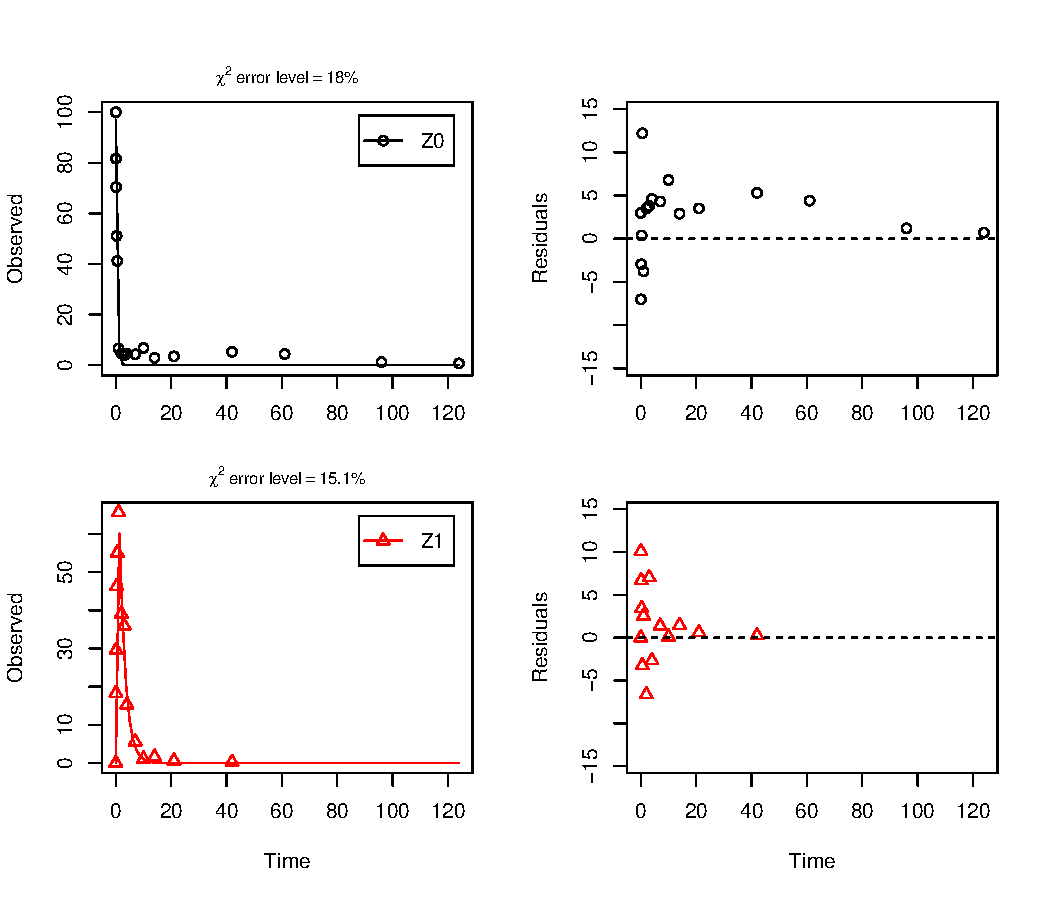
\includegraphics[width=\maxwidth]{figure/FOCUS_2006_Z_fits_1-1} 
\begin{kframe}\begin{alltt}
\hlkwd{summary}\hlstd{(m.Z.2a,} \hlkwc{data} \hlstd{=} \hlnum{FALSE}\hlstd{)}\hlopt{$}\hlstd{bpar}
\end{alltt}
\begin{verbatim}
##               Estimate se_notrans      t value       Pr(>t)
## Z0_0      9.701488e+01 3.55313691 2.730401e+01 1.679214e-21
## k_Z0_sink 1.281376e-11 0.22689470 5.647447e-11 5.000000e-01
## k_Z0_Z1   2.236006e+00 0.16507604 1.354531e+01 7.396594e-14
## k_Z1_sink 4.821248e-01 0.06585369 7.321150e+00 3.552015e-08
##                Lower       Upper
## Z0_0      91.4058170 102.6239462
## k_Z0_sink  0.0000000         Inf
## k_Z0_Z1    1.8419826   2.7143172
## k_Z1_sink  0.4005856   0.5802613
\end{verbatim}
\end{kframe}
\end{knitrout}

As obvious from the parameter summary (the \texttt{bpar} component of the 
summary), the kinetic rate constant from parent compound Z to sink
is negligible. Accordingly, the exact magnitude of the fitted parameter 
\texttt{log k\_Z0\_sink} is ill-defined and the covariance matrix is not
returned (not shown, would be visible in the complete summary). 
This suggests, in agreement with the analysis in the FOCUS kinetics report, to
simplify the model by removing the pathway to sink.

A similar result can be obtained when formation fractions are used in the model 
formulation:

\begin{knitrout}
\definecolor{shadecolor}{rgb}{0.969, 0.969, 0.969}\color{fgcolor}\begin{kframe}
\begin{alltt}
\hlstd{Z.2a.ff} \hlkwb{<-} \hlkwd{mkinmod}\hlstd{(}\hlkwc{Z0} \hlstd{=} \hlkwd{mkinsub}\hlstd{(}\hlstr{"SFO"}\hlstd{,} \hlstr{"Z1"}\hlstd{),}
                   \hlkwc{Z1} \hlstd{=} \hlkwd{mkinsub}\hlstd{(}\hlstr{"SFO"}\hlstd{),}
                   \hlkwc{use_of_ff} \hlstd{=} \hlstr{"max"}\hlstd{)}
\end{alltt}
\begin{verbatim}
## make[1]: warning: jobserver unavailable: using -j1.  Add '+' to parent make rule.
\end{verbatim}


{\ttfamily\noindent\itshape\color{messagecolor}{\#\# Successfully compiled differential equation model from auto-generated C code.}}\begin{alltt}
\hlstd{m.Z.2a.ff} \hlkwb{<-} \hlkwd{mkinfit}\hlstd{(Z.2a.ff, FOCUS_2006_Z_mkin,} \hlkwc{quiet} \hlstd{=} \hlnum{TRUE}\hlstd{)}
\hlkwd{plot_sep}\hlstd{(m.Z.2a.ff)}
\end{alltt}
\end{kframe}
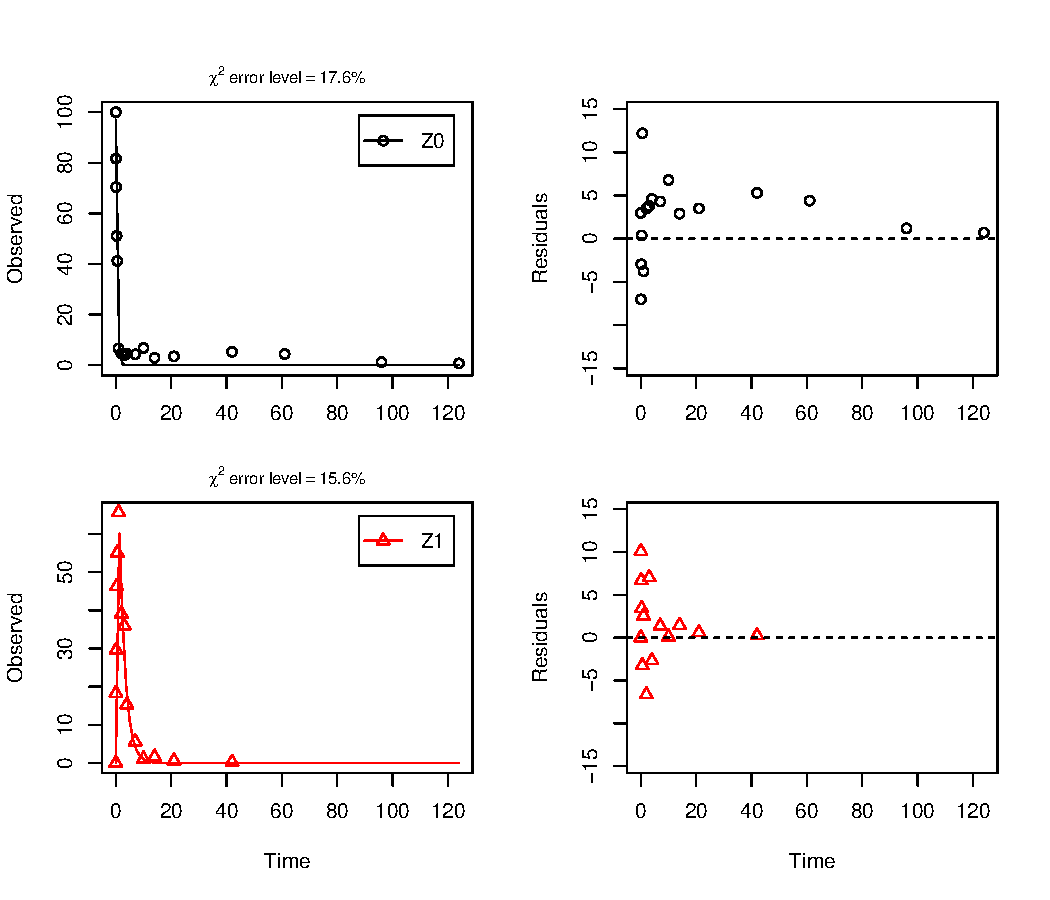
\includegraphics[width=\maxwidth]{figure/FOCUS_2006_Z_fits_2-1} 
\begin{kframe}\begin{alltt}
\hlkwd{summary}\hlstd{(m.Z.2a.ff,} \hlkwc{data} \hlstd{=} \hlnum{FALSE}\hlstd{)}\hlopt{$}\hlstd{bpar}
\end{alltt}
\begin{verbatim}
##              Estimate se_notrans   t value       Pr(>t)      Lower
## Z0_0       97.0148812 3.55314944 27.303912 1.679369e-21 91.3287912
## k_Z0        2.2360064 0.21684747 10.311425 3.661846e-11  1.8052909
## k_Z1        0.4821248 0.06585372  7.321147 3.552045e-08  0.3996826
## f_Z0_to_Z1  1.0000000 0.10147342  9.854798 9.707056e-11  0.0000000
##                  Upper
## Z0_0       102.7009713
## k_Z0         2.7694843
## k_Z1         0.5815722
## f_Z0_to_Z1   1.0000000
\end{verbatim}
\end{kframe}
\end{knitrout}

Here, the ilr transformed formation fraction fitted in the model takes a very
large value, and the backtransformed formation fraction from parent Z to Z1 is
practically unity. Again, the covariance matrix is not returned as the model is
overparameterised. 

The simplified model is obtained by setting the list component \texttt{sink} to
\texttt{FALSE}.\footnote{If the model formulation without formation fractions
is used, the same effect can be obtained by fixing the parameter \texttt{k\_Z\_sink}
to a value of zero.} 

In the following, we use the parameterisation with formation fractions in order
to be able to compare with the results in the FOCUS guidance, and as it 
makes it easier to use parameters obtained in a previous fit when adding a further 
metabolite.

\begin{knitrout}
\definecolor{shadecolor}{rgb}{0.969, 0.969, 0.969}\color{fgcolor}\begin{kframe}
\begin{alltt}
\hlstd{Z.3} \hlkwb{<-} \hlkwd{mkinmod}\hlstd{(}\hlkwc{Z0} \hlstd{=} \hlkwd{mkinsub}\hlstd{(}\hlstr{"SFO"}\hlstd{,} \hlstr{"Z1"}\hlstd{,} \hlkwc{sink} \hlstd{=} \hlnum{FALSE}\hlstd{),}
               \hlkwc{Z1} \hlstd{=} \hlkwd{mkinsub}\hlstd{(}\hlstr{"SFO"}\hlstd{),} \hlkwc{use_of_ff} \hlstd{=} \hlstr{"max"}\hlstd{)}
\end{alltt}
\begin{verbatim}
## make[1]: warning: jobserver unavailable: using -j1.  Add '+' to parent make rule.
\end{verbatim}


{\ttfamily\noindent\itshape\color{messagecolor}{\#\# Successfully compiled differential equation model from auto-generated C code.}}\begin{alltt}
\hlstd{m.Z.3} \hlkwb{<-} \hlkwd{mkinfit}\hlstd{(Z.3, FOCUS_2006_Z_mkin,} \hlkwc{quiet} \hlstd{=} \hlnum{TRUE}\hlstd{)}
\hlkwd{plot_sep}\hlstd{(m.Z.3)}
\end{alltt}
\end{kframe}
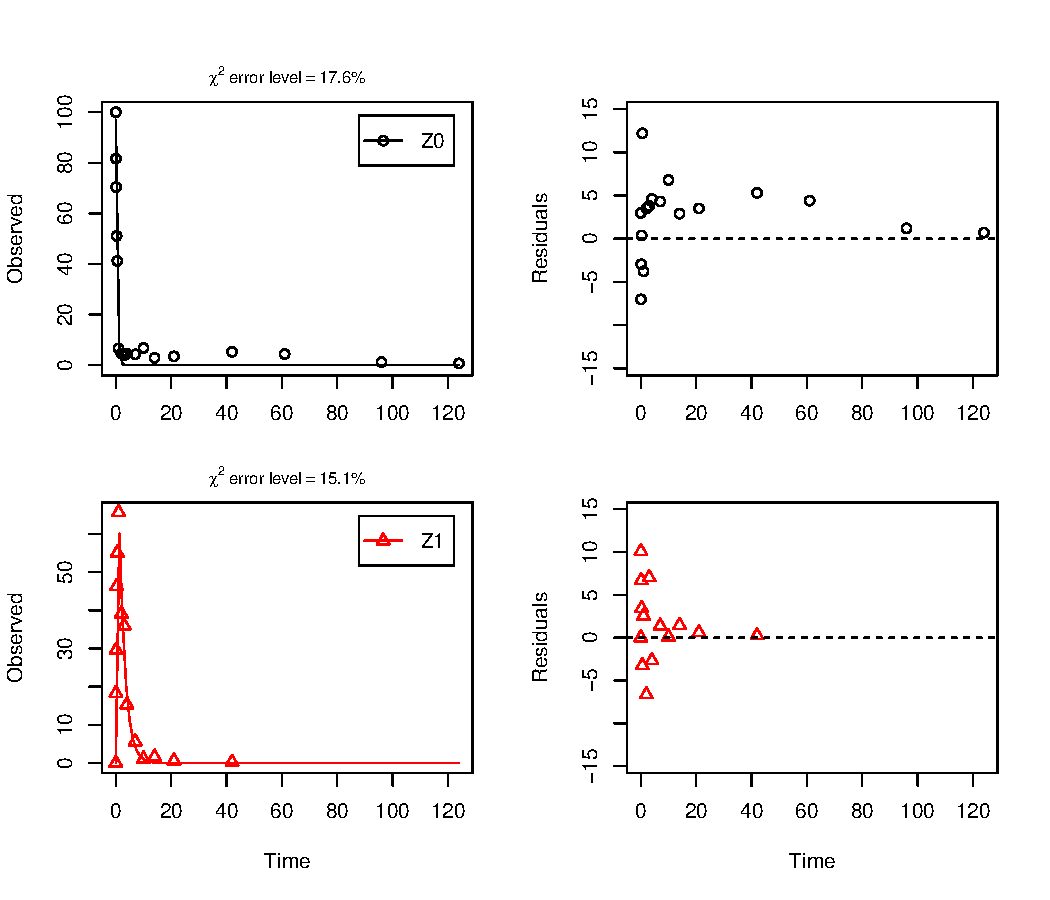
\includegraphics[width=\maxwidth]{figure/FOCUS_2006_Z_fits_3-1} 
\begin{kframe}\begin{alltt}
\hlkwd{summary}\hlstd{(m.Z.3,} \hlkwc{data} \hlstd{=} \hlnum{FALSE}\hlstd{)}\hlopt{$}\hlstd{bpar}
\end{alltt}
\begin{verbatim}
##        Estimate se_notrans  t value       Pr(>t)      Lower
## Z0_0 97.0148815 2.68177093 36.17568 2.363587e-25 91.5215237
## k_Z0  2.2360064 0.14686110 15.22531 2.246514e-15  1.9545310
## k_Z1  0.4821248 0.04268712 11.29439 3.068581e-12  0.4021552
##            Upper
## Z0_0 102.5082392
## k_Z0   2.5580177
## k_Z1   0.5779966
\end{verbatim}
\end{kframe}
\end{knitrout}

As there is only one transformation product for Z0 and no pathway
to sink, the formation fraction is internally fixed to unity.

\section{Including metabolites Z2 and Z3}

As suggested in the FOCUS report, the pathway to sink was removed for metabolite Z1 as
well in the next step. While this step appears questionable on the basis of the above results, it 
is followed here for the purpose of comparison. Also, in the FOCUS report, it is 
assumed that there is additional empirical evidence that Z1 quickly and exclusively
hydrolyses to Z2. 

\begin{knitrout}
\definecolor{shadecolor}{rgb}{0.969, 0.969, 0.969}\color{fgcolor}\begin{kframe}
\begin{alltt}
\hlstd{Z.5} \hlkwb{<-} \hlkwd{mkinmod}\hlstd{(}\hlkwc{Z0} \hlstd{=} \hlkwd{mkinsub}\hlstd{(}\hlstr{"SFO"}\hlstd{,} \hlstr{"Z1"}\hlstd{,} \hlkwc{sink} \hlstd{=} \hlnum{FALSE}\hlstd{),}
               \hlkwc{Z1} \hlstd{=} \hlkwd{mkinsub}\hlstd{(}\hlstr{"SFO"}\hlstd{,} \hlstr{"Z2"}\hlstd{,} \hlkwc{sink} \hlstd{=} \hlnum{FALSE}\hlstd{),}
               \hlkwc{Z2} \hlstd{=} \hlkwd{mkinsub}\hlstd{(}\hlstr{"SFO"}\hlstd{),} \hlkwc{use_of_ff} \hlstd{=} \hlstr{"max"}\hlstd{)}
\end{alltt}
\begin{verbatim}
## make[1]: warning: jobserver unavailable: using -j1.  Add '+' to parent make rule.
\end{verbatim}


{\ttfamily\noindent\itshape\color{messagecolor}{\#\# Successfully compiled differential equation model from auto-generated C code.}}\begin{alltt}
\hlstd{m.Z.5} \hlkwb{<-} \hlkwd{mkinfit}\hlstd{(Z.5, FOCUS_2006_Z_mkin,} \hlkwc{quiet} \hlstd{=} \hlnum{TRUE}\hlstd{)}
\hlkwd{plot_sep}\hlstd{(m.Z.5)}
\end{alltt}
\end{kframe}
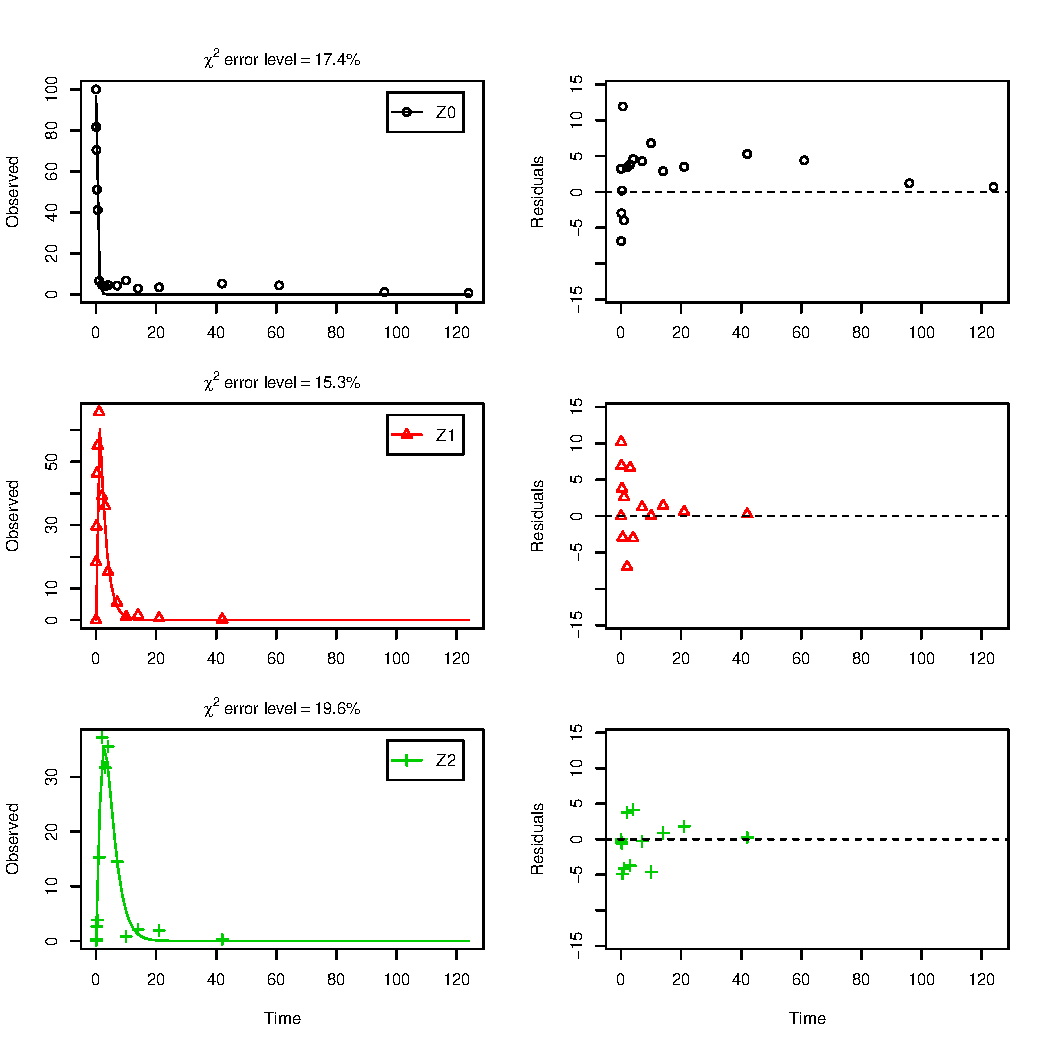
\includegraphics[width=\maxwidth]{figure/FOCUS_2006_Z_fits_5-1} 

\end{knitrout}

Finally, metabolite Z3 is added to the model. We use the optimised
differential equation parameter values from the previous fit in order to
accelerate the optimization.

\begin{knitrout}
\definecolor{shadecolor}{rgb}{0.969, 0.969, 0.969}\color{fgcolor}\begin{kframe}
\begin{alltt}
\hlstd{Z.FOCUS} \hlkwb{<-} \hlkwd{mkinmod}\hlstd{(}\hlkwc{Z0} \hlstd{=} \hlkwd{mkinsub}\hlstd{(}\hlstr{"SFO"}\hlstd{,} \hlstr{"Z1"}\hlstd{,} \hlkwc{sink} \hlstd{=} \hlnum{FALSE}\hlstd{),}
                   \hlkwc{Z1} \hlstd{=} \hlkwd{mkinsub}\hlstd{(}\hlstr{"SFO"}\hlstd{,} \hlstr{"Z2"}\hlstd{,} \hlkwc{sink} \hlstd{=} \hlnum{FALSE}\hlstd{),}
                   \hlkwc{Z2} \hlstd{=} \hlkwd{mkinsub}\hlstd{(}\hlstr{"SFO"}\hlstd{,} \hlstr{"Z3"}\hlstd{),}
                   \hlkwc{Z3} \hlstd{=} \hlkwd{mkinsub}\hlstd{(}\hlstr{"SFO"}\hlstd{),}
                   \hlkwc{use_of_ff} \hlstd{=} \hlstr{"max"}\hlstd{)}
\end{alltt}
\begin{verbatim}
## make[1]: warning: jobserver unavailable: using -j1.  Add '+' to parent make rule.
\end{verbatim}


{\ttfamily\noindent\itshape\color{messagecolor}{\#\# Successfully compiled differential equation model from auto-generated C code.}}\begin{alltt}
\hlstd{m.Z.FOCUS} \hlkwb{<-} \hlkwd{mkinfit}\hlstd{(Z.FOCUS, FOCUS_2006_Z_mkin,}
                     \hlkwc{parms.ini} \hlstd{= m.Z.5}\hlopt{$}\hlstd{bparms.ode,}
                     \hlkwc{quiet} \hlstd{=} \hlnum{TRUE}\hlstd{)}
\hlkwd{plot_sep}\hlstd{(m.Z.FOCUS)}
\end{alltt}
\end{kframe}
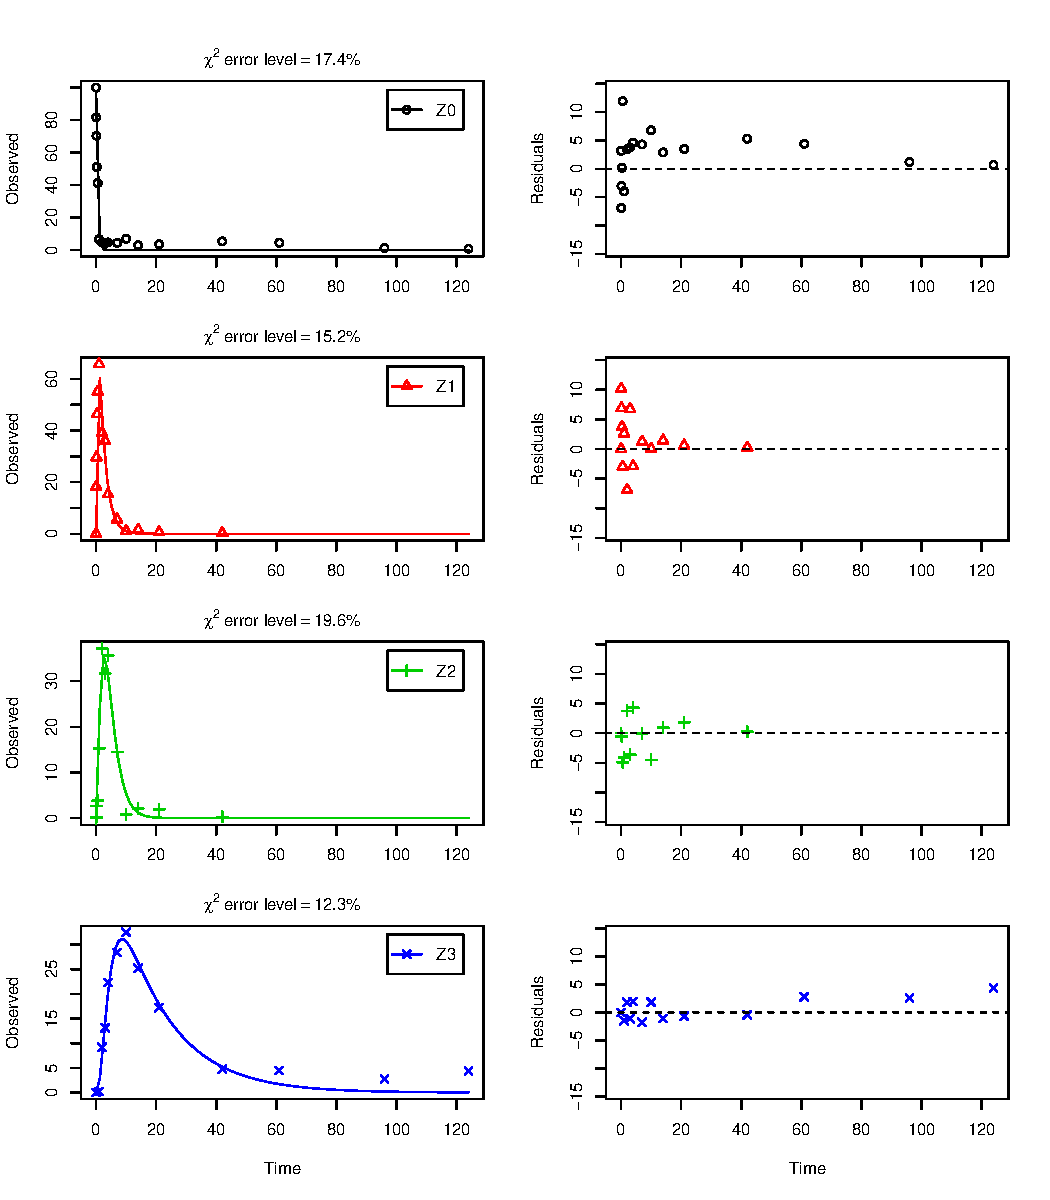
\includegraphics[width=\maxwidth]{figure/FOCUS_2006_Z_fits_6-1} 
\begin{kframe}\begin{alltt}
\hlkwd{summary}\hlstd{(m.Z.FOCUS,} \hlkwc{data} \hlstd{=} \hlnum{FALSE}\hlstd{)}\hlopt{$}\hlstd{bpar}
\end{alltt}
\begin{verbatim}
##               Estimate se_notrans   t value       Pr(>t)       Lower
## Z0_0       96.83849566 2.05886133 47.034977 5.583742e-44 92.70517559
## k_Z0        2.21540897 0.11813046 18.753919 7.744034e-25  1.99051134
## k_Z1        0.47829896 0.02928763 16.331089 3.333376e-22  0.42297603
## k_Z2        0.45161653 0.04421268 10.214638 3.110936e-14  0.37103495
## k_Z3        0.05869343 0.01429485  4.105914 7.285393e-05  0.03599566
## f_Z2_to_Z3  0.47150952 0.05705233  8.264510 2.809889e-11  0.36038193
##                   Upper
## Z0_0       100.97181573
## k_Z0         2.46571661
## k_Z1         0.54085782
## k_Z2         0.54969886
## k_Z3         0.09570371
## f_Z2_to_Z3   0.58553462
\end{verbatim}
\begin{alltt}
\hlkwd{endpoints}\hlstd{(m.Z.FOCUS)}
\end{alltt}
\begin{verbatim}
## $ff
##     Z2_Z3   Z2_sink 
## 0.4715095 0.5284905 
## 
## $SFORB
## logical(0)
## 
## $distimes
##          DT50      DT90
## Z0  0.3128755  1.039350
## Z1  1.4491923  4.814113
## Z2  1.5348136  5.098540
## Z3 11.8096217 39.230714
\end{verbatim}
\end{kframe}
\end{knitrout}

This fit corresponds to the final result chosen in Appendix 7 of the FOCUS
report. Confidence intervals returned by mkin are based on internally
transformed parameters, however.

\section{Using the SFORB model for parent and metabolites}

As the FOCUS report states, there is a certain tailing of the time course of metabolite 
Z3. Also, the time course of the parent compound is not fitted very well using the 
SFO model, as residues at a certain low level remain.

Therefore, an additional model is offered here, using the single first-order 
reversible binding (SFORB) model for metabolite Z3. As expected, the $\chi^2$
error level is lower for metabolite Z3 using this model and the graphical 
fit for Z3 is improved. However, the covariance matrix is not returned.

\begin{knitrout}
\definecolor{shadecolor}{rgb}{0.969, 0.969, 0.969}\color{fgcolor}\begin{kframe}
\begin{alltt}
\hlstd{Z.mkin.1} \hlkwb{<-} \hlkwd{mkinmod}\hlstd{(}\hlkwc{Z0} \hlstd{=} \hlkwd{mkinsub}\hlstd{(}\hlstr{"SFO"}\hlstd{,} \hlstr{"Z1"}\hlstd{,} \hlkwc{sink} \hlstd{=} \hlnum{FALSE}\hlstd{),}
                    \hlkwc{Z1} \hlstd{=} \hlkwd{mkinsub}\hlstd{(}\hlstr{"SFO"}\hlstd{,} \hlstr{"Z2"}\hlstd{,} \hlkwc{sink} \hlstd{=} \hlnum{FALSE}\hlstd{),}
                    \hlkwc{Z2} \hlstd{=} \hlkwd{mkinsub}\hlstd{(}\hlstr{"SFO"}\hlstd{,} \hlstr{"Z3"}\hlstd{),}
                    \hlkwc{Z3} \hlstd{=} \hlkwd{mkinsub}\hlstd{(}\hlstr{"SFORB"}\hlstd{))}
\end{alltt}
\begin{verbatim}
## make[1]: warning: jobserver unavailable: using -j1.  Add '+' to parent make rule.
\end{verbatim}


{\ttfamily\noindent\itshape\color{messagecolor}{\#\# Successfully compiled differential equation model from auto-generated C code.}}\begin{alltt}
\hlstd{m.Z.mkin.1} \hlkwb{<-} \hlkwd{mkinfit}\hlstd{(Z.mkin.1, FOCUS_2006_Z_mkin,} \hlkwc{quiet} \hlstd{=} \hlnum{TRUE}\hlstd{)}
\hlkwd{plot_sep}\hlstd{(m.Z.mkin.1)}
\end{alltt}
\end{kframe}
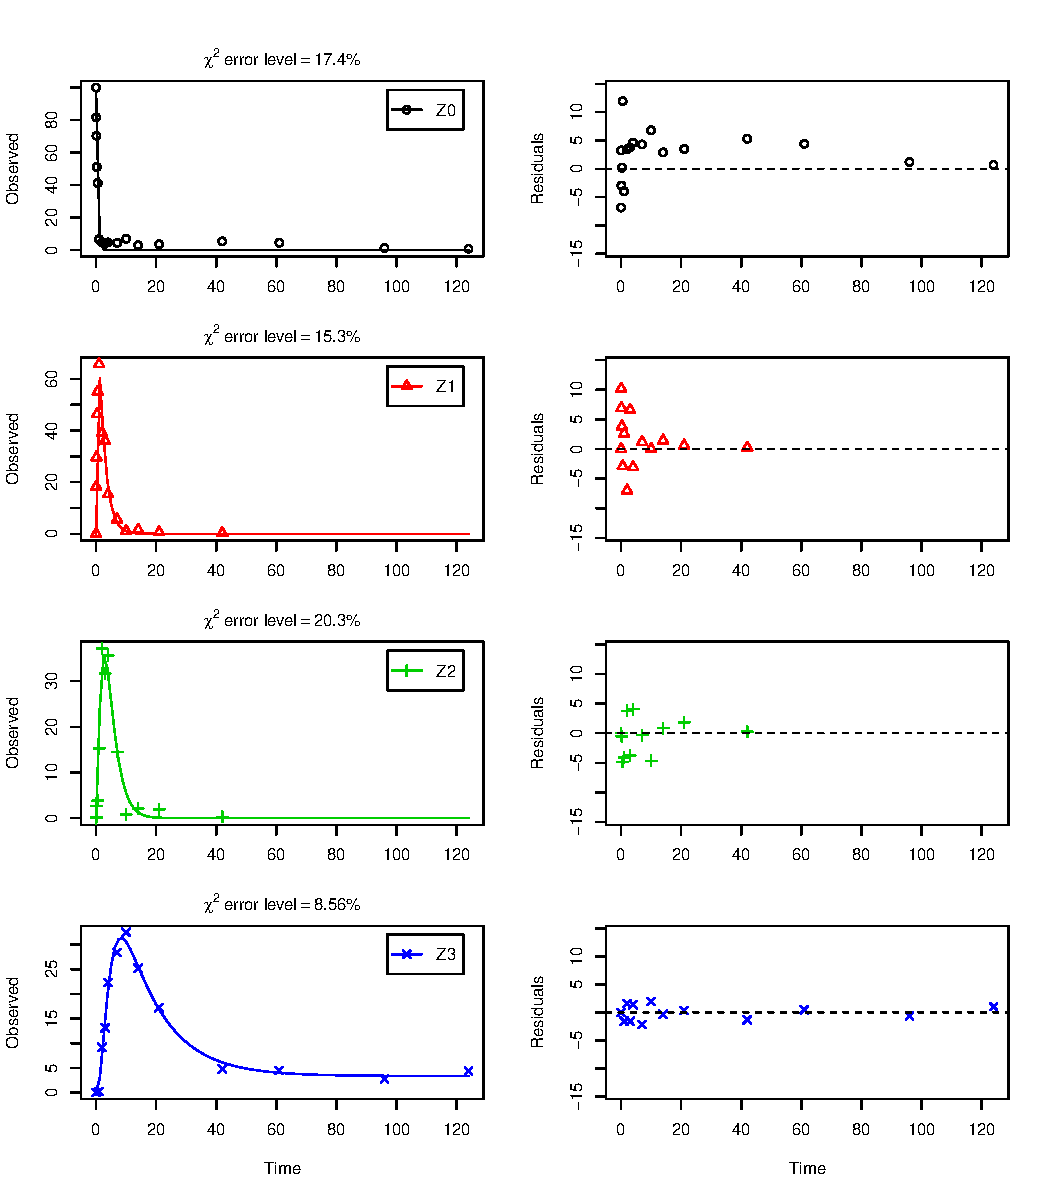
\includegraphics[width=\maxwidth]{figure/FOCUS_2006_Z_fits_7-1} 
\begin{kframe}\begin{alltt}
\hlkwd{summary}\hlstd{(m.Z.mkin.1,} \hlkwc{data} \hlstd{=} \hlnum{FALSE}\hlstd{)}\hlopt{$}\hlstd{cov.unscaled}
\end{alltt}
\begin{verbatim}
## NULL
\end{verbatim}
\end{kframe}
\end{knitrout}

Therefore, a further stepwise model building is performed starting from the
stage of parent and two metabolites, starting from the assumption that the model
fit for the parent compound can be improved by using the SFORB model.

\begin{knitrout}
\definecolor{shadecolor}{rgb}{0.969, 0.969, 0.969}\color{fgcolor}\begin{kframe}
\begin{alltt}
\hlstd{Z.mkin.3} \hlkwb{<-} \hlkwd{mkinmod}\hlstd{(}\hlkwc{Z0} \hlstd{=} \hlkwd{mkinsub}\hlstd{(}\hlstr{"SFORB"}\hlstd{,} \hlstr{"Z1"}\hlstd{,} \hlkwc{sink} \hlstd{=} \hlnum{FALSE}\hlstd{),}
                    \hlkwc{Z1} \hlstd{=} \hlkwd{mkinsub}\hlstd{(}\hlstr{"SFO"}\hlstd{,} \hlstr{"Z2"}\hlstd{,} \hlkwc{sink} \hlstd{=} \hlnum{FALSE}\hlstd{),}
                    \hlkwc{Z2} \hlstd{=} \hlkwd{mkinsub}\hlstd{(}\hlstr{"SFO"}\hlstd{))}
\end{alltt}
\begin{verbatim}
## make[1]: warning: jobserver unavailable: using -j1.  Add '+' to parent make rule.
\end{verbatim}


{\ttfamily\noindent\itshape\color{messagecolor}{\#\# Successfully compiled differential equation model from auto-generated C code.}}\begin{alltt}
\hlstd{m.Z.mkin.3} \hlkwb{<-} \hlkwd{mkinfit}\hlstd{(Z.mkin.3, FOCUS_2006_Z_mkin,} \hlkwc{quiet} \hlstd{=} \hlnum{TRUE}\hlstd{)}
\hlkwd{plot_sep}\hlstd{(m.Z.mkin.3)}
\end{alltt}
\end{kframe}
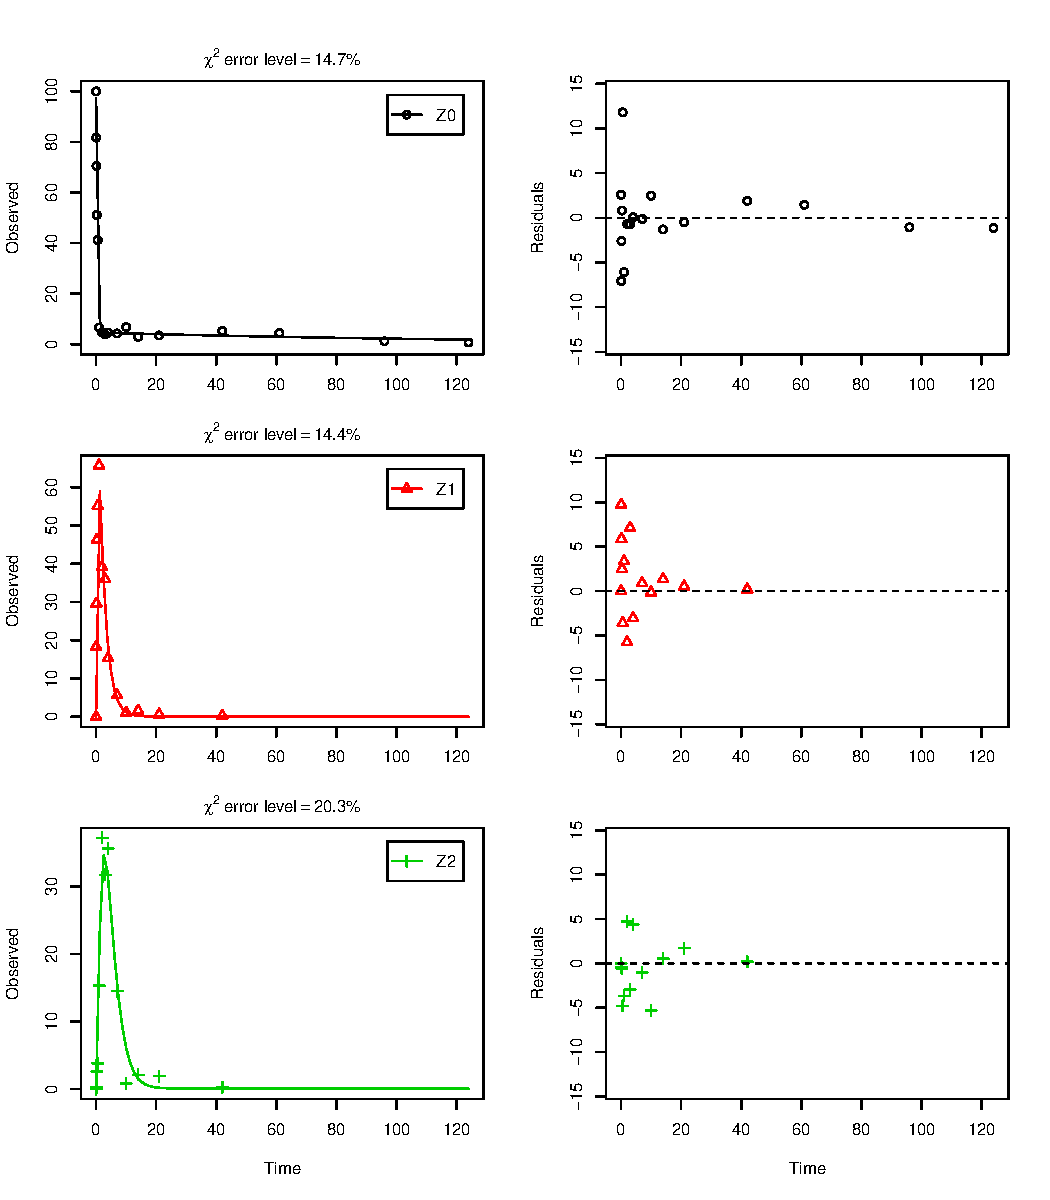
\includegraphics[width=\maxwidth]{figure/FOCUS_2006_Z_fits_9-1} 

\end{knitrout}

This results in a much better representation of the behaviour of the parent 
compound Z0.

Finally, Z3 is added as well. These models appear overparameterised (no
covariance matrix returned) if the sink for Z1 is left in the models.

\begin{knitrout}
\definecolor{shadecolor}{rgb}{0.969, 0.969, 0.969}\color{fgcolor}\begin{kframe}
\begin{alltt}
\hlstd{Z.mkin.4} \hlkwb{<-} \hlkwd{mkinmod}\hlstd{(}\hlkwc{Z0} \hlstd{=} \hlkwd{mkinsub}\hlstd{(}\hlstr{"SFORB"}\hlstd{,} \hlstr{"Z1"}\hlstd{,} \hlkwc{sink} \hlstd{=} \hlnum{FALSE}\hlstd{),}
                    \hlkwc{Z1} \hlstd{=} \hlkwd{mkinsub}\hlstd{(}\hlstr{"SFO"}\hlstd{,} \hlstr{"Z2"}\hlstd{,} \hlkwc{sink} \hlstd{=} \hlnum{FALSE}\hlstd{),}
                    \hlkwc{Z2} \hlstd{=} \hlkwd{mkinsub}\hlstd{(}\hlstr{"SFO"}\hlstd{,} \hlstr{"Z3"}\hlstd{),}
                    \hlkwc{Z3} \hlstd{=} \hlkwd{mkinsub}\hlstd{(}\hlstr{"SFO"}\hlstd{))}
\end{alltt}
\begin{verbatim}
## make[1]: warning: jobserver unavailable: using -j1.  Add '+' to parent make rule.
\end{verbatim}


{\ttfamily\noindent\itshape\color{messagecolor}{\#\# Successfully compiled differential equation model from auto-generated C code.}}\begin{alltt}
\hlstd{m.Z.mkin.4} \hlkwb{<-} \hlkwd{mkinfit}\hlstd{(Z.mkin.4, FOCUS_2006_Z_mkin,}
                      \hlkwc{parms.ini} \hlstd{= m.Z.mkin.3}\hlopt{$}\hlstd{bparms.ode,}
                      \hlkwc{quiet} \hlstd{=} \hlnum{TRUE}\hlstd{)}
\hlkwd{plot_sep}\hlstd{(m.Z.mkin.4)}
\end{alltt}
\end{kframe}
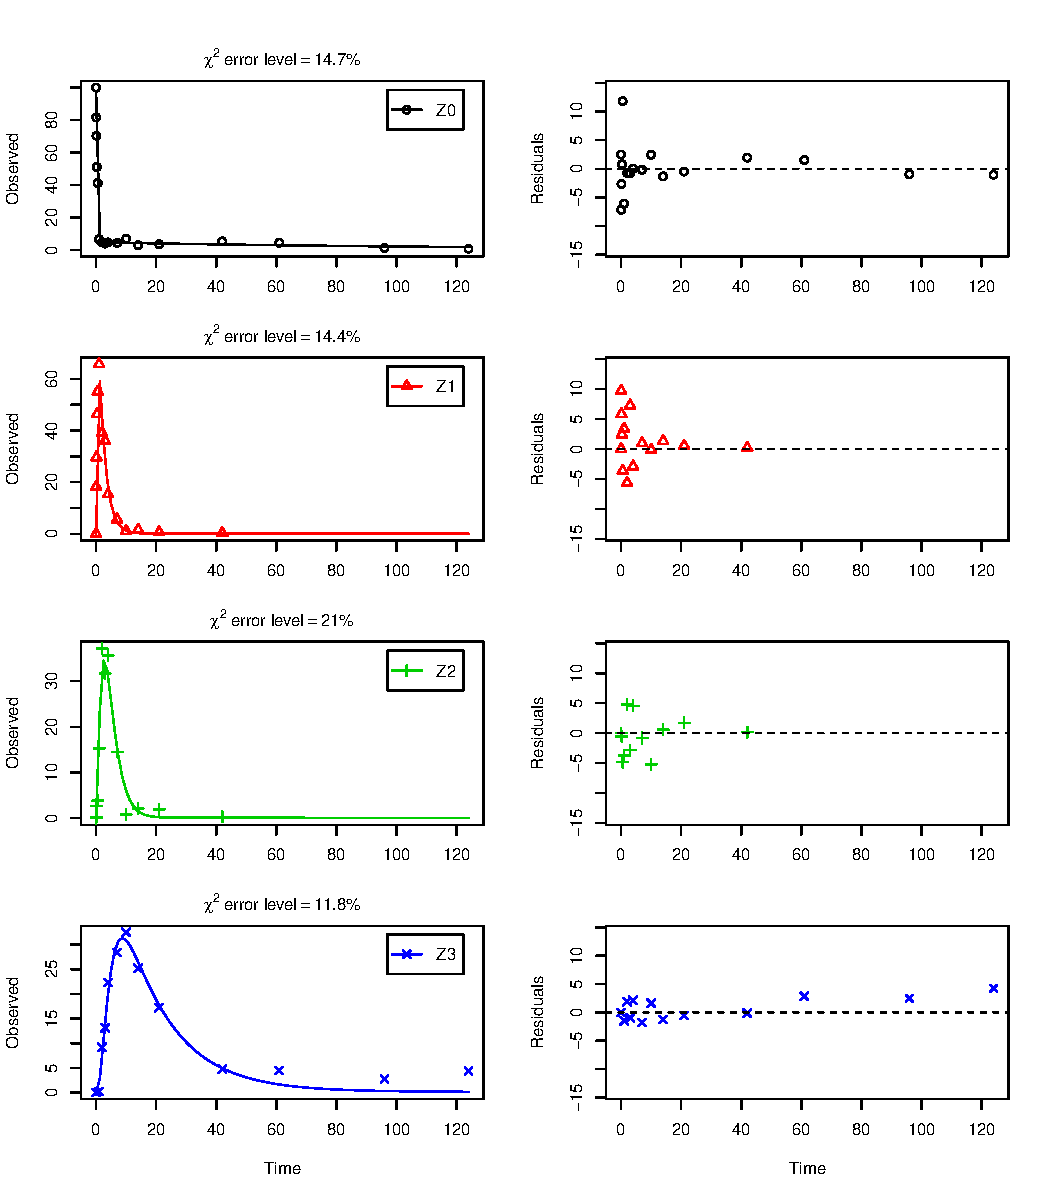
\includegraphics[width=\maxwidth]{figure/FOCUS_2006_Z_fits_10-1} 

\end{knitrout}

The error level of the fit, but especially of metabolite Z3, can be improved if
the SFORB model is chosen for this metabolite, as this model is capable of
representing the tailing of the metabolite decline phase.

\begin{knitrout}
\definecolor{shadecolor}{rgb}{0.969, 0.969, 0.969}\color{fgcolor}\begin{kframe}
\begin{alltt}
\hlstd{Z.mkin.5} \hlkwb{<-} \hlkwd{mkinmod}\hlstd{(}\hlkwc{Z0} \hlstd{=} \hlkwd{mkinsub}\hlstd{(}\hlstr{"SFORB"}\hlstd{,} \hlstr{"Z1"}\hlstd{,} \hlkwc{sink} \hlstd{=} \hlnum{FALSE}\hlstd{),}
                    \hlkwc{Z1} \hlstd{=} \hlkwd{mkinsub}\hlstd{(}\hlstr{"SFO"}\hlstd{,} \hlstr{"Z2"}\hlstd{,} \hlkwc{sink} \hlstd{=} \hlnum{FALSE}\hlstd{),}
                    \hlkwc{Z2} \hlstd{=} \hlkwd{mkinsub}\hlstd{(}\hlstr{"SFO"}\hlstd{,} \hlstr{"Z3"}\hlstd{),}
                    \hlkwc{Z3} \hlstd{=} \hlkwd{mkinsub}\hlstd{(}\hlstr{"SFORB"}\hlstd{))}
\end{alltt}
\begin{verbatim}
## make[1]: warning: jobserver unavailable: using -j1.  Add '+' to parent make rule.
\end{verbatim}


{\ttfamily\noindent\itshape\color{messagecolor}{\#\# Successfully compiled differential equation model from auto-generated C code.}}\begin{alltt}
\hlstd{m.Z.mkin.5} \hlkwb{<-} \hlkwd{mkinfit}\hlstd{(Z.mkin.5, FOCUS_2006_Z_mkin,}
                      \hlkwc{parms.ini} \hlstd{= m.Z.mkin.4}\hlopt{$}\hlstd{bparms.ode[}\hlnum{1}\hlopt{:}\hlnum{4}\hlstd{],}
                      \hlkwc{quiet} \hlstd{=} \hlnum{TRUE}\hlstd{)}
\hlkwd{plot_sep}\hlstd{(m.Z.mkin.5)}
\end{alltt}
\end{kframe}
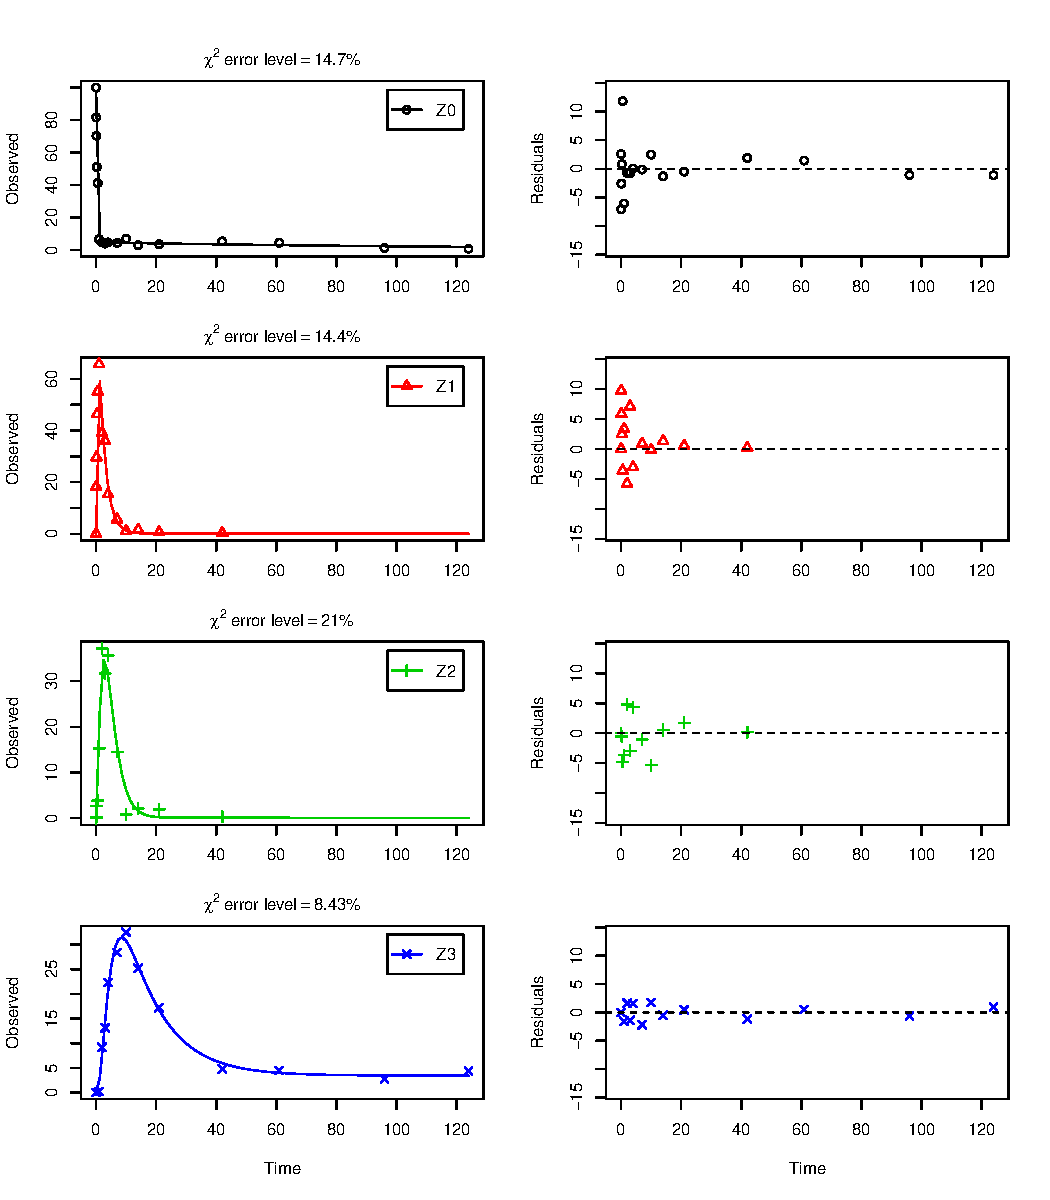
\includegraphics[width=\maxwidth]{figure/FOCUS_2006_Z_fits_11-1} 

\end{knitrout}

The summary view of the backtransformed parameters shows that we get no
confidence intervals due to overparameterisation. As the optimized
\texttt{k\_Z3\_bound\_free} is excessively small, it seems reasonable to fix it to
zero. 

\begin{knitrout}
\definecolor{shadecolor}{rgb}{0.969, 0.969, 0.969}\color{fgcolor}\begin{kframe}
\begin{alltt}
\hlstd{m.Z.mkin.5a} \hlkwb{<-} \hlkwd{mkinfit}\hlstd{(Z.mkin.5, FOCUS_2006_Z_mkin,}
                       \hlkwc{parms.ini} \hlstd{=} \hlkwd{c}\hlstd{(m.Z.mkin.5}\hlopt{$}\hlstd{bparms.ode[}\hlnum{1}\hlopt{:}\hlnum{7}\hlstd{],}
                                     \hlkwc{k_Z3_bound_free} \hlstd{=} \hlnum{0}\hlstd{),}
                       \hlkwc{fixed_parms} \hlstd{=} \hlstr{"k_Z3_bound_free"}\hlstd{,}
                       \hlkwc{quiet} \hlstd{=} \hlnum{TRUE}\hlstd{)}
\hlkwd{plot_sep}\hlstd{(m.Z.mkin.5a)}
\end{alltt}
\end{kframe}
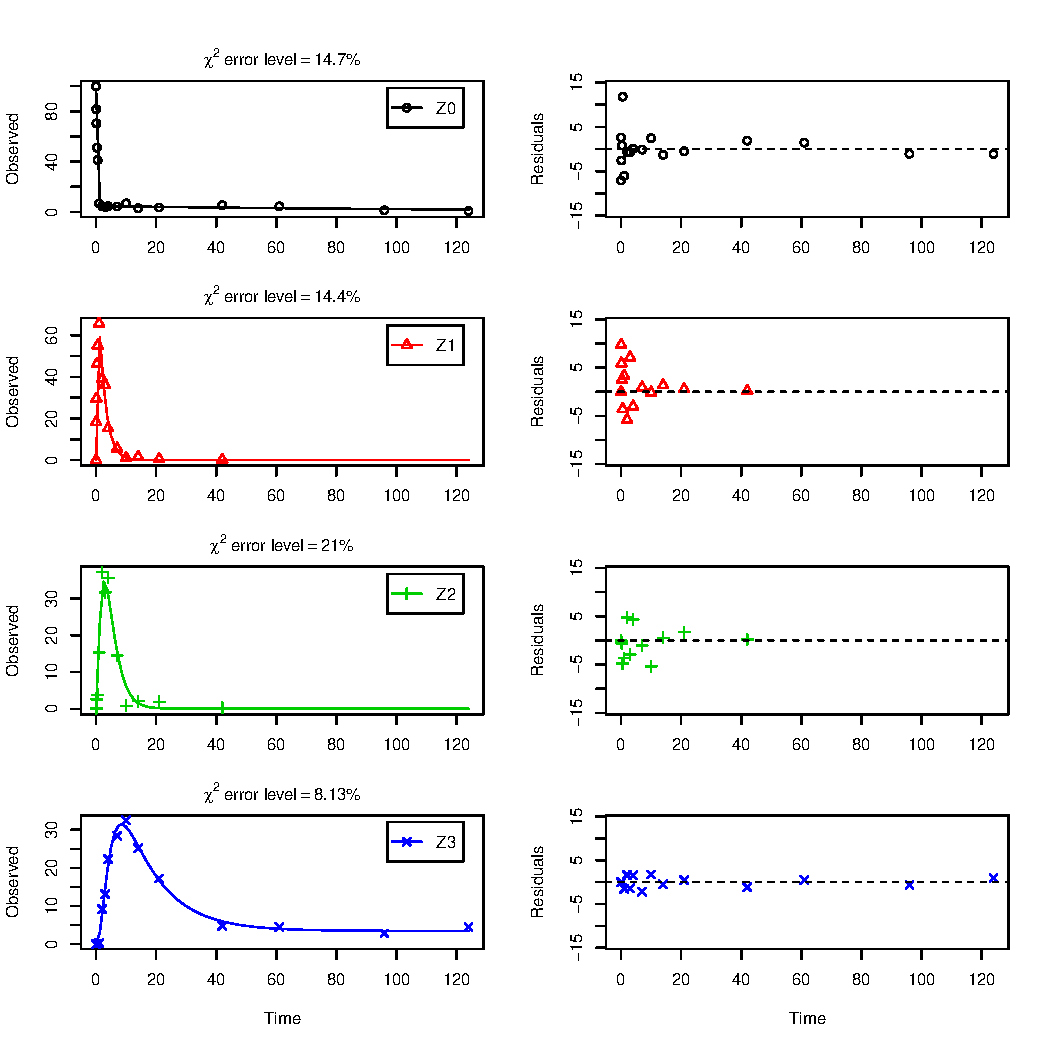
\includegraphics[width=\maxwidth]{figure/FOCUS_2006_Z_fits_11a-1} 

\end{knitrout}

As expected, the residual plots for Z0 and Z3 are more random than in the case of the 
all SFO model for which they were shown above. In conclusion, the model
\texttt{Z.mkin.5a} is proposed as the best-fit model for the dataset from
Appendix 7 of the FOCUS report.

A graphical representation of the confidence intervals can finally be obtained.

\begin{knitrout}
\definecolor{shadecolor}{rgb}{0.969, 0.969, 0.969}\color{fgcolor}\begin{kframe}
\begin{alltt}
\hlkwd{mkinparplot}\hlstd{(m.Z.mkin.5a)}
\end{alltt}
\end{kframe}
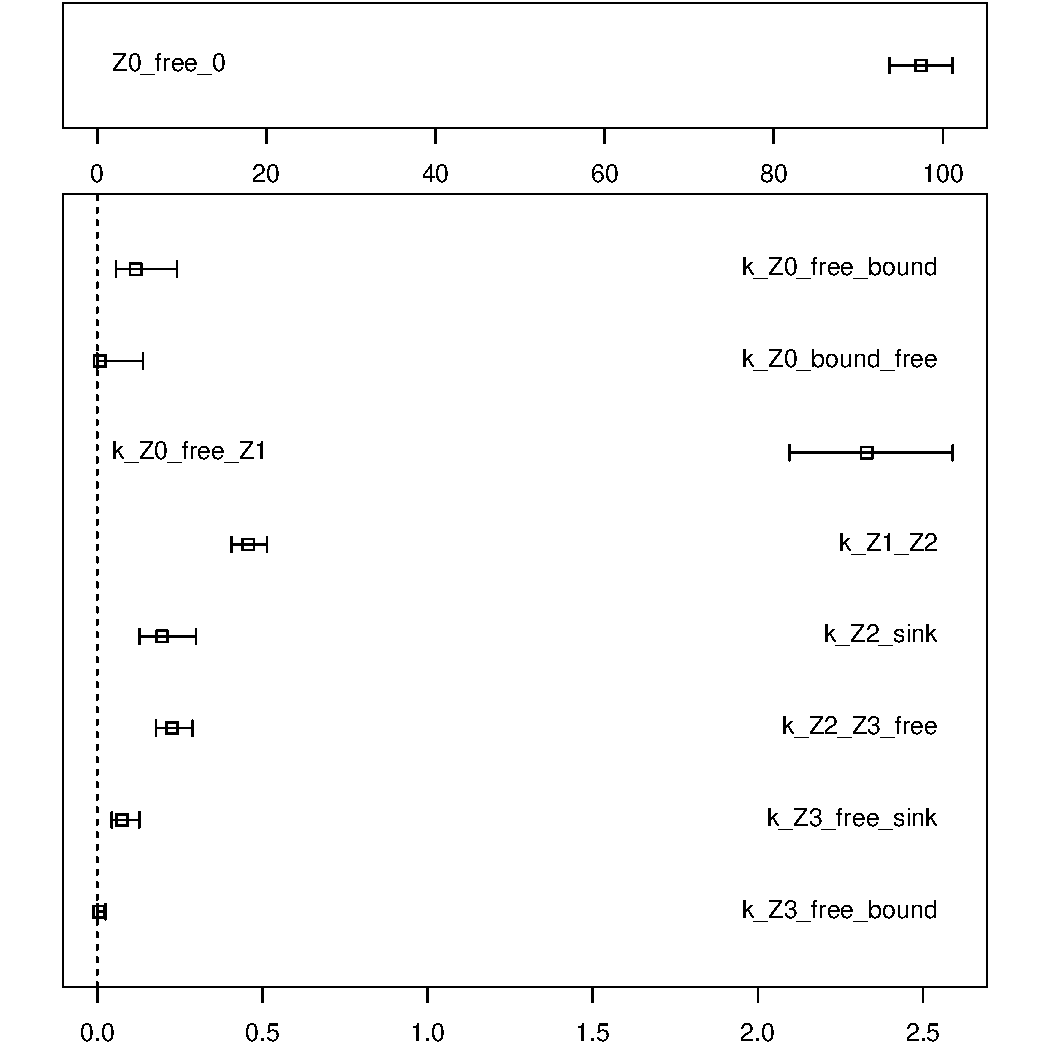
\includegraphics[width=\maxwidth]{figure/FOCUS_2006_Z_fits_11b-1} 

\end{knitrout}

The endpoints obtained with this model are

\begin{knitrout}
\definecolor{shadecolor}{rgb}{0.969, 0.969, 0.969}\color{fgcolor}\begin{kframe}
\begin{alltt}
\hlkwd{endpoints}\hlstd{(m.Z.mkin.5a)}
\end{alltt}
\begin{verbatim}
## $ff
##   Z0_free_Z1        Z1_Z2      Z2_sink   Z2_Z3_free Z3_free_sink 
##    1.0000000    1.0000000    0.4634431    0.5365569    1.0000000 
## 
## $SFORB
##       Z0_b1       Z0_b2       Z3_b1       Z3_b2 
## 2.447138640 0.007512589 0.080007099 0.000000000 
## 
## $distimes
##         DT50     DT90 DT50_Z0_b1 DT50_Z0_b2 DT50_Z3_b1 DT50_Z3_b2
## Z0 0.3042972 1.184811   0.283248   92.26476         NA         NA
## Z1 1.5147787 5.031986         NA         NA         NA         NA
## Z2 1.6413857 5.452565         NA         NA         NA         NA
## Z3        NA       NA         NA         NA   8.663571        Inf
\end{verbatim}
\end{kframe}
\end{knitrout}

It is clear the degradation rate of Z3 towards the end of the experiment 
is very low as DT50\_Z3\_b2 (the second Eigenvalue of the system of two differential 
equations representing the SFORB system for Z3, corresponding to the slower rate
constant of the DFOP model) is reported to be infinity.  However, this appears
to be a feature of the data.

\bibliographystyle{plainnat}
\bibliography{references}

\end{document}
% vim: set foldmethod=syntax:
